\part{Concepts Fondamentaux }
\chapter{Reconnaissance des panneaux de signalisation routière}
\label{chap:premierchapitre}
\minitoc

Dans ce chapitre, nous allons voir des généralités sur les panneaux de signalisation routière ainsi que différentes applications des systèmes de détection et de reconnaissance automatiques tout en entamant les étapes principales du processus de la reconnaissance.

\section{Panneaux de signalisation routière}

Les panneaux de signalisation routière constituent un élément important de la circulation routière. Leur fonction principale est d’exposer et d’afficher le contenu qui doit avertir les conducteur des dangers potentiels ainsi que les informations sur la route. C’est pour cette raison que la détection et l’identification des panneaux de signalisation est un aspect de recherche très important dans la prévention des accidents au niveau de route (Figure- \ref{fig: panneaux-al}).

\begin{figure}[htp!]
     \centering
      \begin{subfigure}
          \centering    
              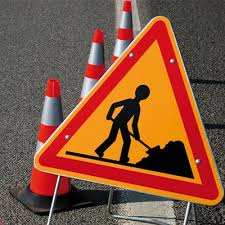
\includegraphics[width=3.5cm,height=4cm]{images/ii.jpg}
              \end{subfigure}
           \hfill
     \begin{subfigure}
              \centering  
       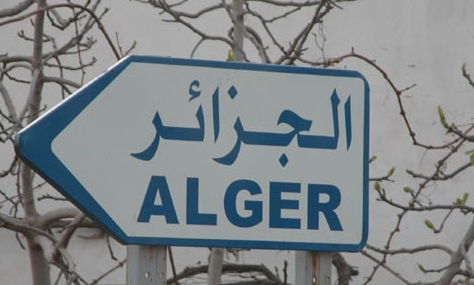
\includegraphics[width=3.5cm,height=4cm]{images/300.jpg}
     \end{subfigure}
          \hfill
     \begin{subfigure}
             \centering     
            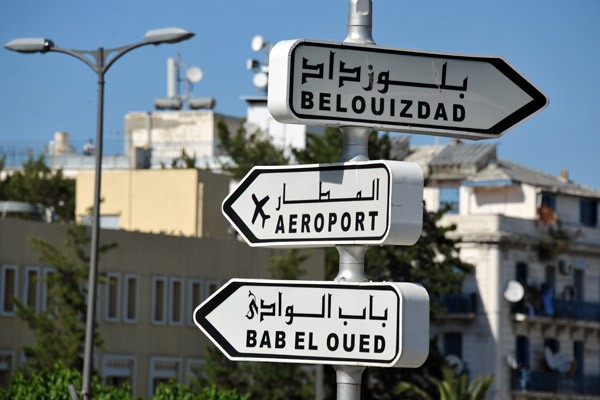
\includegraphics[width=3.5cm,height=4cm]{images/3.jpg}
     \end{subfigure}
           \hfill
     \begin{subfigure}
              \centering    
            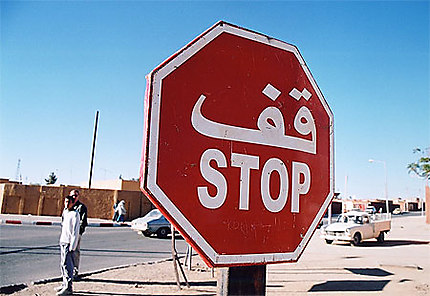
\includegraphics[width=3.5cm,height=4cm]{images/5.jpg}
     \end{subfigure}
      \caption{Exemples de plaques routières en Algérie}
       \label{fig: panneaux-al}
\end{figure}

\subsection{Classification des panneaux de signalisation routière }

Une convention sur la signalisation routière a été faite à Vienne le 8 novembre 1968. Cette dernière consiste en un  traité international qui a réuni un ensemble de pays (Figure- \ref{fig:participants de Viennes}), reconnaissant que l’uniformité et la normalisation des panneaux de signalisation, des feux de circulation de routes et des marquages, sont nécessaires pour gérer la circulation routière. \cite{1}.\\

\begin{figure}[h!]
        \centering
        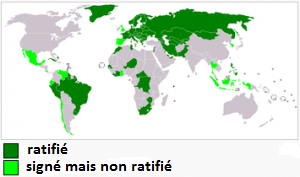
\includegraphics[width=8cm,height=4cm]{images/vienna.png}
        \caption{Participants à l’union de Vienne}
        \label{fig:participants de Viennes}
\end{figure}
    
A partir de cette réunion, plusieurs  articles ont été fournis parmi lesquelles l’article numéro "02" qui classe les panneaux de signalisation routière en catégories nommées de ‘A’  à ‘H’ contenant chacune un groupe de panneaux spécifiques (Tableau-\ref{table:classes de panneaux}).\\
Les sections principales issues de l’article sont:
\begin{table}[]
\centering
\begin{tabular}{|l|l|l|}
\hline
\multicolumn{1}{|c|}{code de la section} & \multicolumn{1}{|c|}{contenu} & \multicolumn{1}{|c|}{exemple}  \\ \hline
  \multicolumn{1}{|c|}{A }
  & 
  \multicolumn{1}{|c|}{Les panneaux d'avertissement de danger} 
  & 
 \multicolumn{1}{|c|}{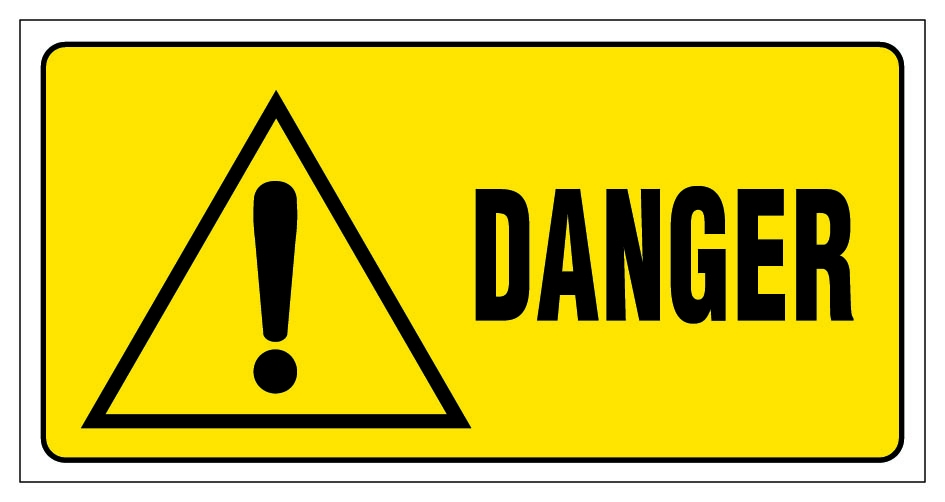
\includegraphics[width=2.5cm,height=2cm]{100.jpg}}   \\ \hline
  \multicolumn{1}{|c|}{B}    &
\multicolumn{1}{|c|}{Les signes de priorité} 
& \multicolumn{1}{|c|}{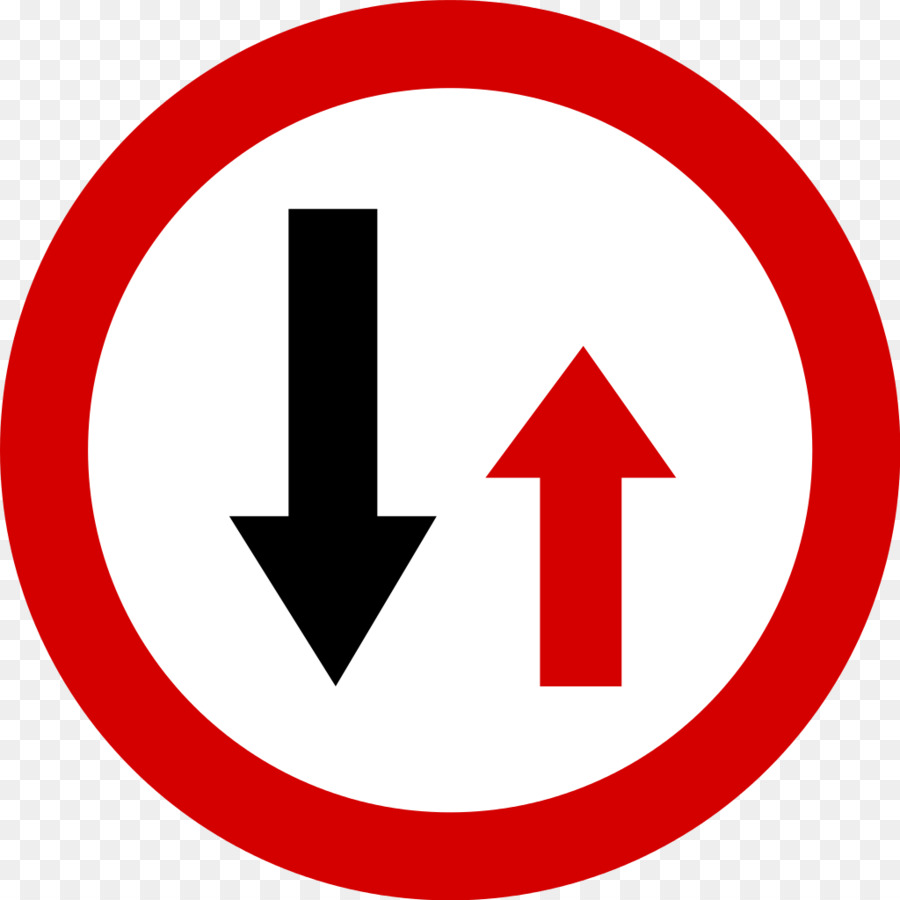
\includegraphics[width=2.5cm,height=2cm]{101.jpg}} \\ \hline
 \multicolumn{1}{|c|}  {C}  
    & 
 \multicolumn{1}{|c|}   {Les signes d'interdiction ou de restriction}   & 
 \multicolumn{1}{|c|}  {
\includegraphics[width=2.5cm,height=2cm]{102.jpg} }\\ \hline
     \multicolumn{1}{|c|} {D} 
    & 
    \multicolumn{1}{|c|}{Les signes obligatoires}
    & 
     \multicolumn{1}{|c|} {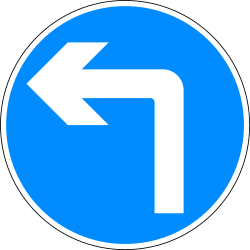
\includegraphics[width=2.5cm,height=2cm]{103.png}}  \\ \hline
      \multicolumn{1}{|c|}{E}  
    & 
    \multicolumn{1}{|c|}{Signalisation réglementaire spéciale}  
    & 
 \multicolumn{1}{|c|} {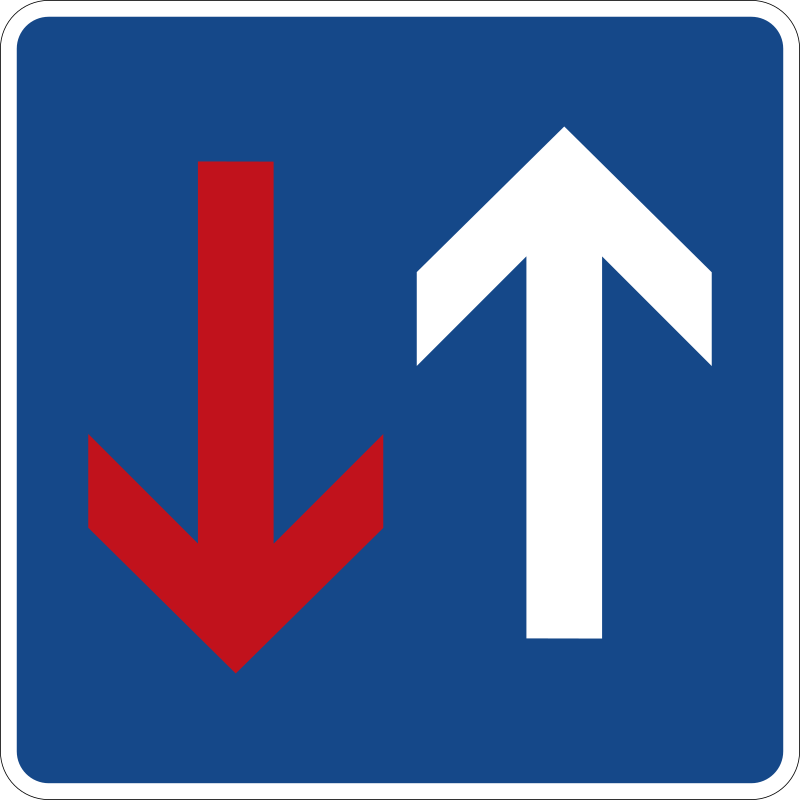
\includegraphics[width=2.5cm,height=2cm]{sss.png}} \\  \hline  
  \multicolumn{1}{|c|} {F}   
    & 
    \multicolumn{1}{|c|}{Informations, installations ou panneaux de service} 
    & 
    \multicolumn{1}{|c|}{
\includegraphics[width=2.5cm,height=2cm]{exit.png}} \\      \hline 
   \multicolumn{1}{|c|}{G}
    & 
   \multicolumn{1}{|c|} {Panneau de direction, de position ou d'indication}
    & 
   \multicolumn{1}{|c|}{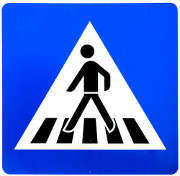
\includegraphics[width=2.5cm,height=2cm]{104.jpg}} \\       \hline   
   \multicolumn{1}{|c|}{H } 
    & 
    \multicolumn{1}{|c|}{Panneaux supplémentaires} 
    & 
    \multicolumn{1}{|c|}{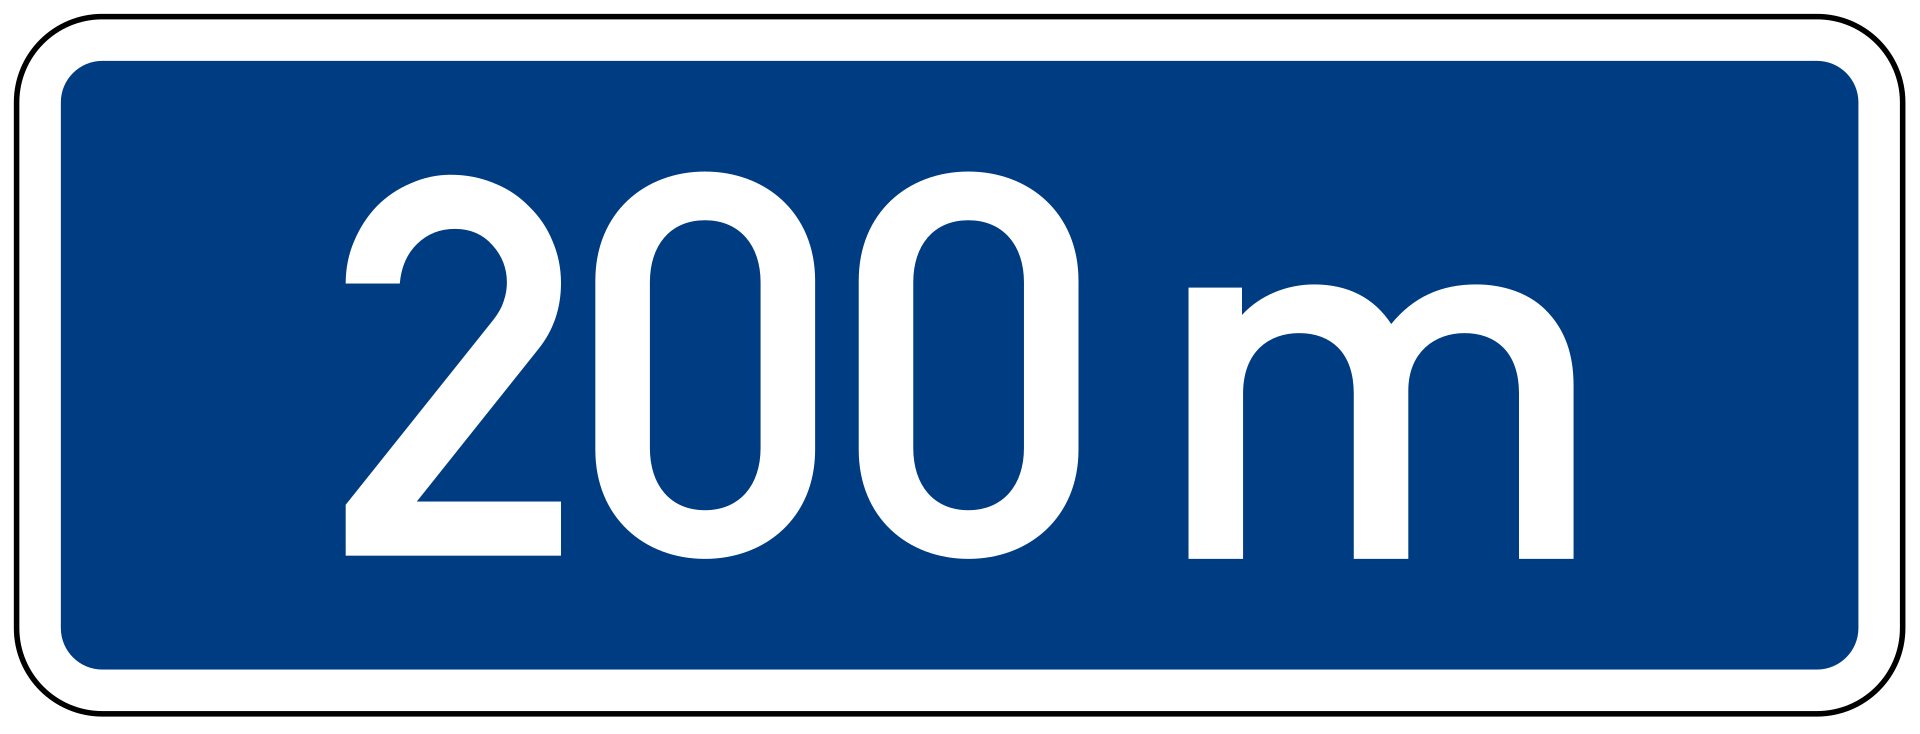
\includegraphics[width=2.5cm,height=2cm]{images/200.png}} \\  \hline   
         
\end{tabular}
\caption{Classes de panneaux de signalisation routière}
\label{table:classes de panneaux}
\end{table}
\newpage
La convention, dans une deuxième partie, définit les couleurs, des tailles et des formes précises pour chacune de ces classes de signes.\\
Malgré les normalisations et les standards qui furent révisés plusieurs fois, il existe toujours des différences entre les pays contractés dans l’accord. Le tableau (Table-\ref{table:diff-p}) montre des panneaux indiquant la présence d'un passage piéton dans différents pays.\\
\begin{table}[]
\centering
\begin{tabular}{|l|l|l|}
\hline
\multicolumn{1}{|c|}{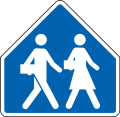
\includegraphics[width=3cm,height=2.5cm]{images/pieton5.png}} & \multicolumn{1}{c|}{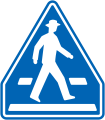
\includegraphics[width=3cm,height=2.5cm]{images/pieton3.png}} & \multicolumn{1}{c|}{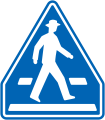
\includegraphics[width=3cm,height=2.5cm]{images/pieton3.png}} \\ \hline
\multicolumn{1}{|c|}{En Malaisie}    & \multicolumn{1}{c|}{Au Japon }  & \multicolumn{1}{c|}{Aux Philippines}\\ \hline
\end{tabular}
\caption{Exemple de différence entre les panneaux de         signalisation routière}
\label{table:diff-p}
\end{table}
\subsection{Propriétés des panneaux de signalisations routière}

Les panneaux de signalisation ont été conçus pour être distincts des arrières plans naturels ou artificiels et ils ont des caractéristiques qui les rendent reconnaissables dans l’environnement. En général, ils sont fabriqués et installés conformément à des règles strictes (Figure- \ref{fig:formes}).
Les symboles sur les panneaux ont une couleur qui les distingue de l'arrière plan de la scène. La teinte de la peinture qui recouvre le signe correspond à une longueur d'onde spécifique dans le spectre visible. Les panneaux sont situés à des emplacements bien définis sur la route, de sorte que le conducteur peut s’attendre à les observer. Ils  peuvent contenir des pictogrammes, du texte ou les deux au même temps tout en prenant une forme géométrique particulière (cercle,triangle, rectangle, etc.)
\begin{figure}[h]
  \centering
  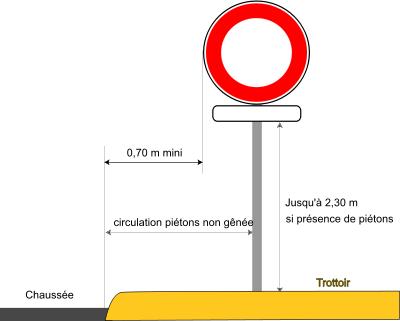
\includegraphics[width=7cm,height=5cm]{images/rte.png}
  \caption{Exemple de différentes règles d'implantations d'un panneau routier}
  \label{fig:formes}
\end{figure}

\newpage
\section{Domaines d’application}

La détection et la reconnaissance des panneaux de signalisation routière a prouvée un grand intérêt au cours des dernières années,cela est dû au large éventail d'applications qu'un système doté de cette capacité offre;

\subsection{Entretien des autoroutes}

Quotidiennement, un opérateur humain doit  vérifier la présence et l'état des panneaux au niveau des autoroutes (Figure-\ref{fig:entretien}).\\

\begin{figure}[h]
        \centering
        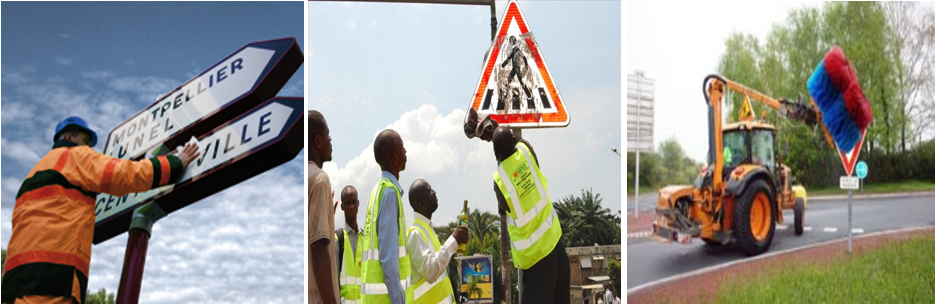
\includegraphics[width=10cm,height=3cm]{images/ccc.png}
        \caption{Entretien de panneaux routiers}
        \label{fig:entretien}
\end{figure}

C'est une tâche fastidieuse car les panneaux sont nombreux. Il y a un projet européen appelé "AUTOCAT" \cite{2} qui présente une fourgonnette développée pour la collecte automatique de la position et l'orientation des panneaux de signalisation routière (Figure- \ref{fig:vehicules de}) ci-dessus montre des véhicules modernes dans le même contexte.

\begin{figure}[h]
        \centering
        \begin{subfigure}
        \centering
        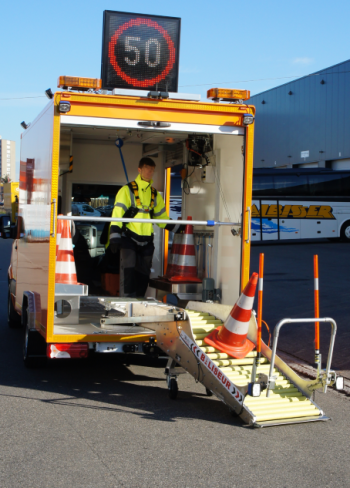
\includegraphics[width=4cm,height=4cm]{images/c1.png}  \end{subfigure}
         \begin{subfigure}
         \centering
        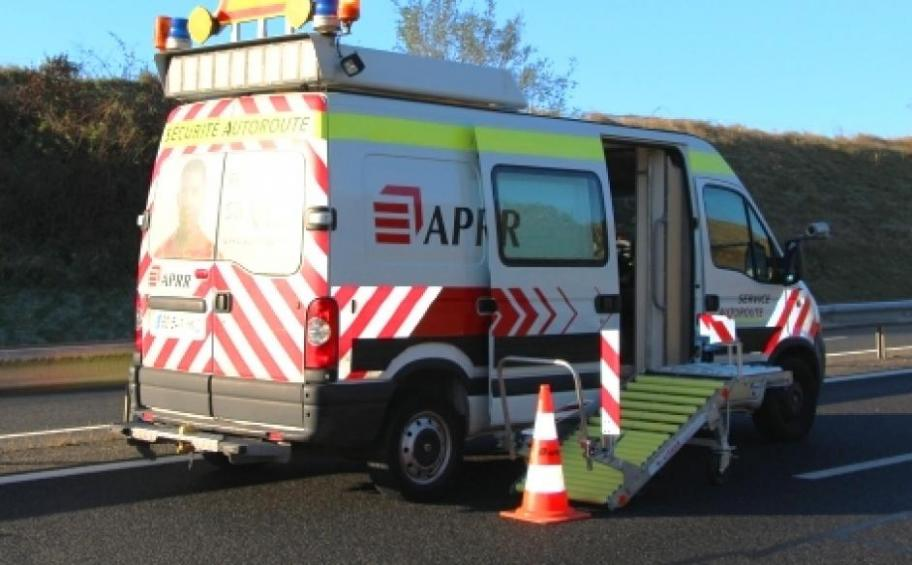
\includegraphics[width=4cm,height=4cm]{images/c2.png}
        \end{subfigure}
        \begin{subfigure}
        \centering
        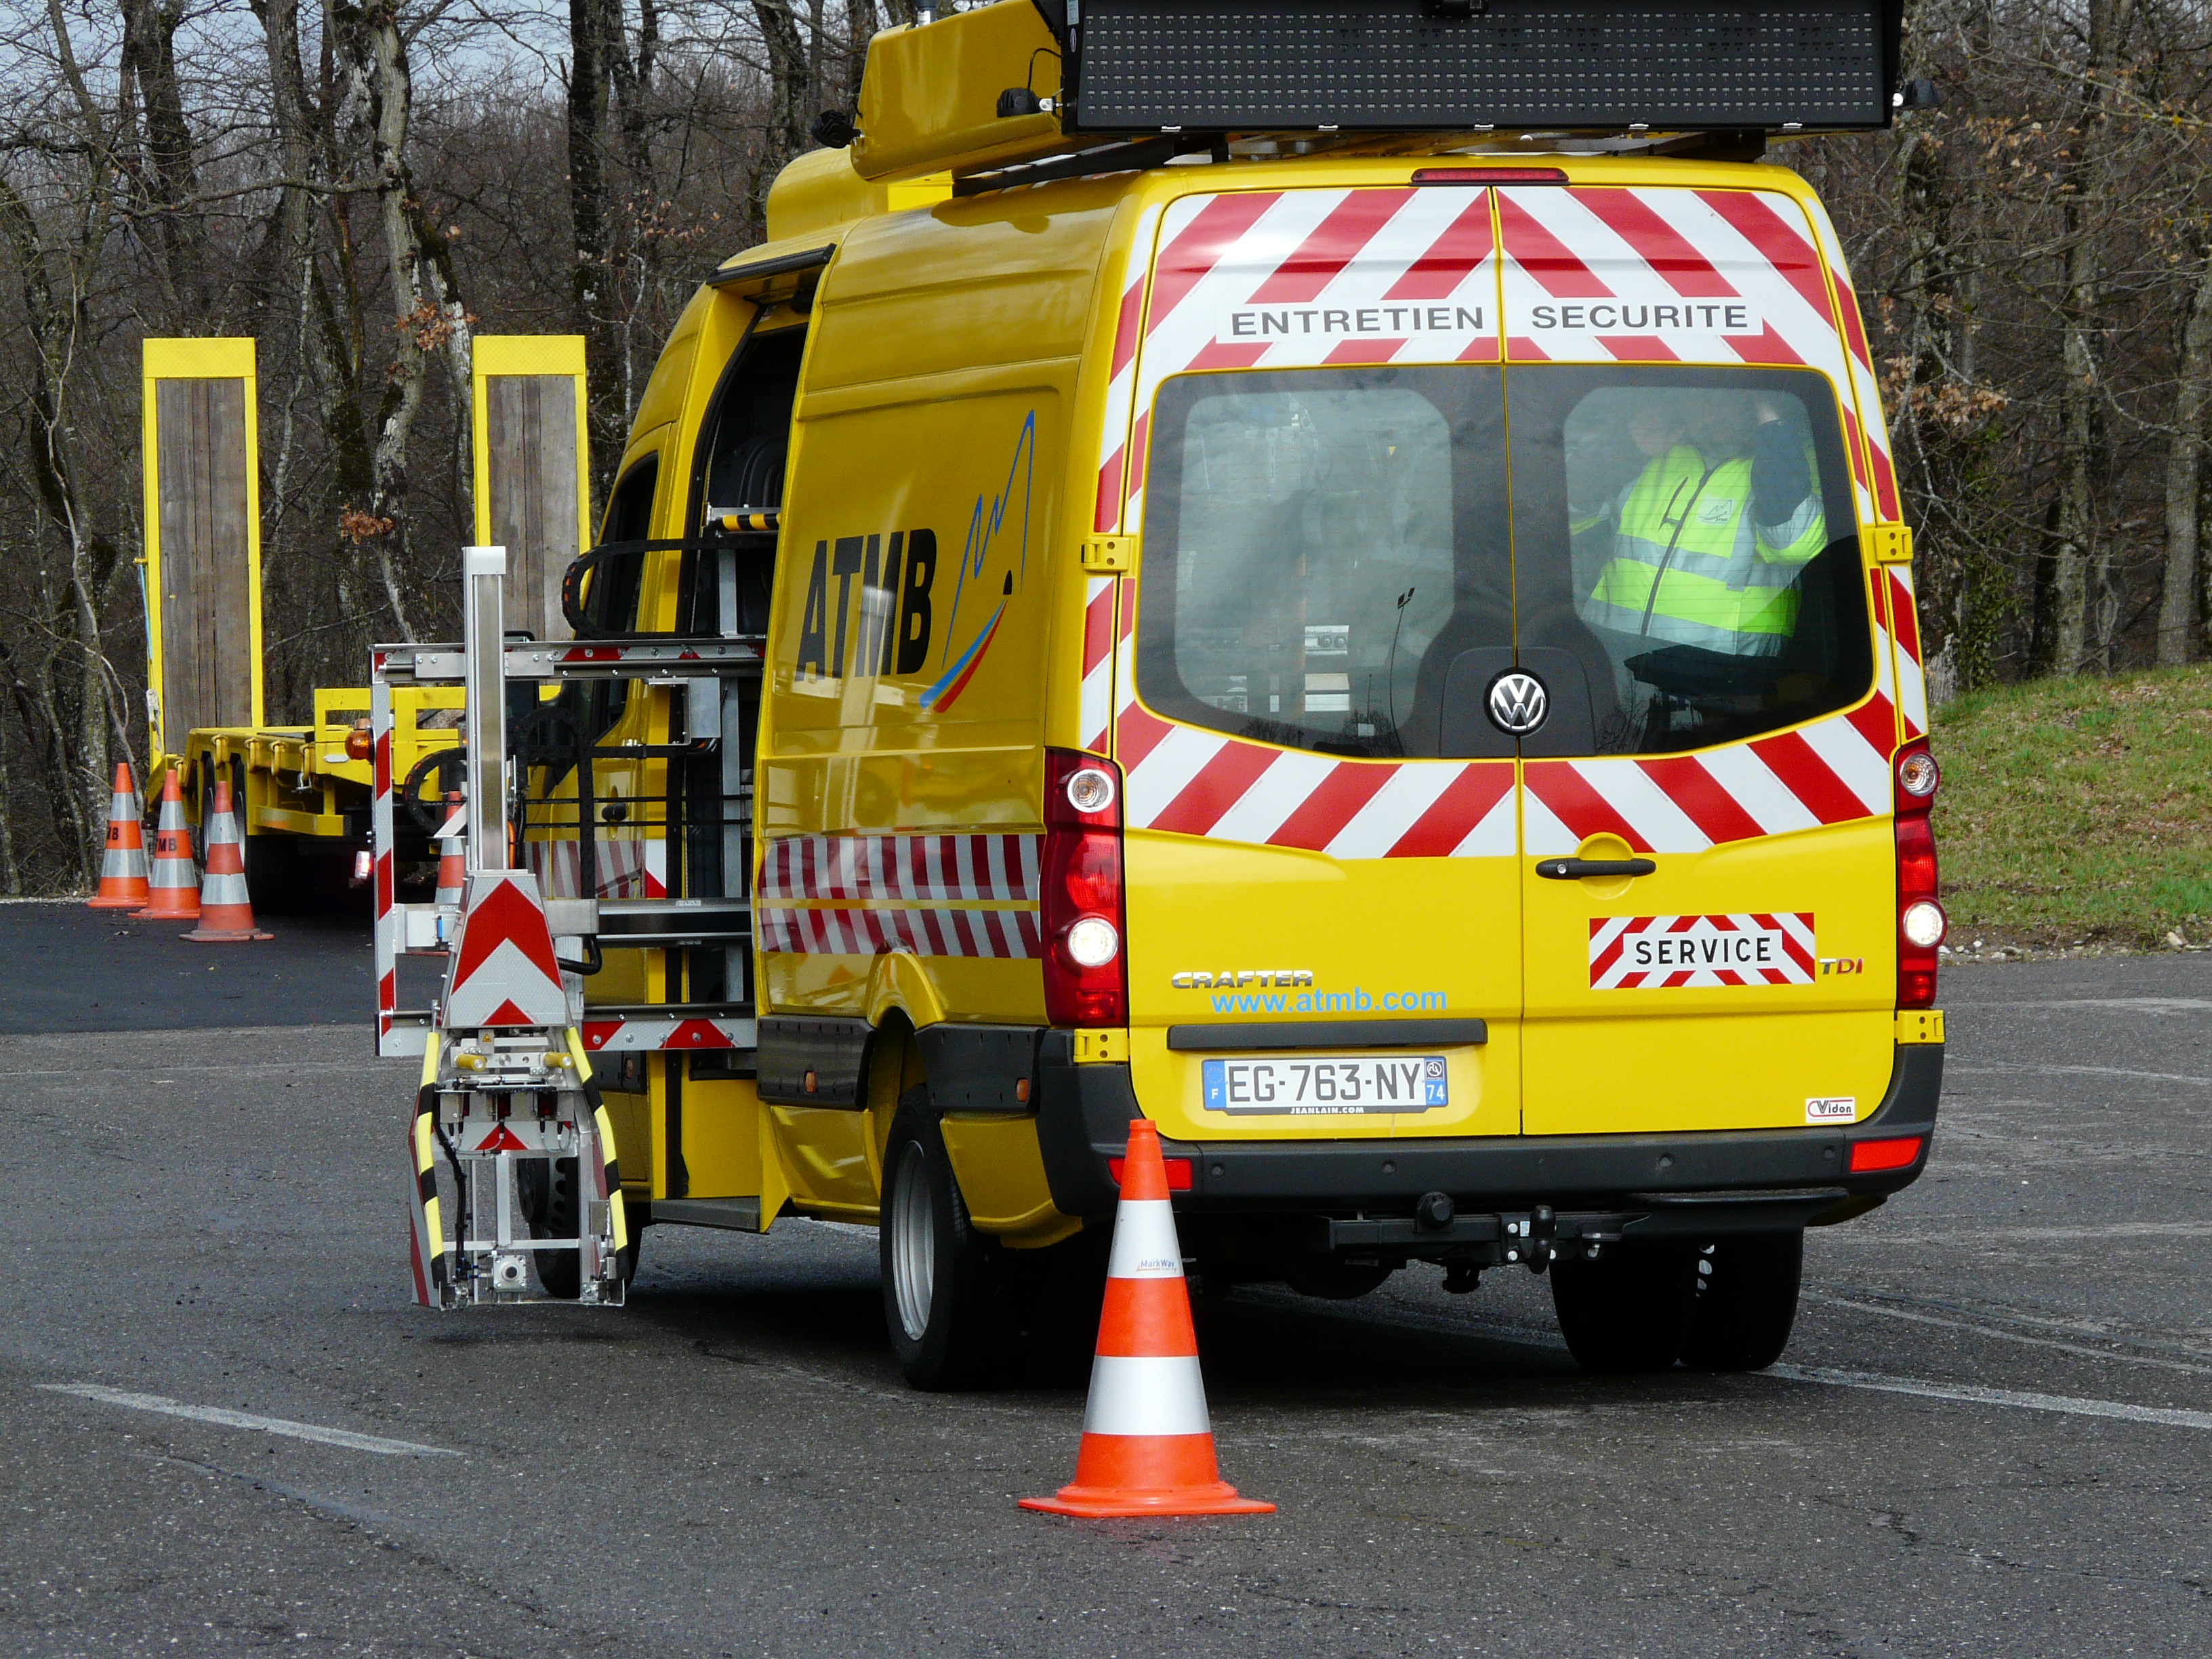
\includegraphics[width=4cm,height=4cm]{images/c4.jpg} \end{subfigure}
        \caption{Véhicules de démonstration modernes}
        \label{fig:vehicules de}
\end{figure}
    
\subsection{Inventaire de signes routiers}

L'inventaire en général se fait dans les villes ou l'environnement est plus complexe que les autoroutes. ils ne sont pas toujours placés perpendiculairement au sol.

\subsection{Systèmes d'assistance aux conducteurs}

Ces systèmes informent ou assistent le conducteur afin d’éviter l’apparition de danger (Figure-\ref{fig:systeme intelligents}).
Il y a des groupes de recherche qui se sont concentrés sur des aspects liés au développement d'un pilote automatique, tels que :
\begin{itemize}
  \item La détection des frontières de la route \cite{3,4} ;
    \item La reconnaissance d'obstacles sur la trajectoire du véhicule tels que d'autres véhicules ou piétons \cite{5,6,7}.
  \end{itemize}
 \vspace{0.5cm} 
 \begin{figure}[h]
        \centering
        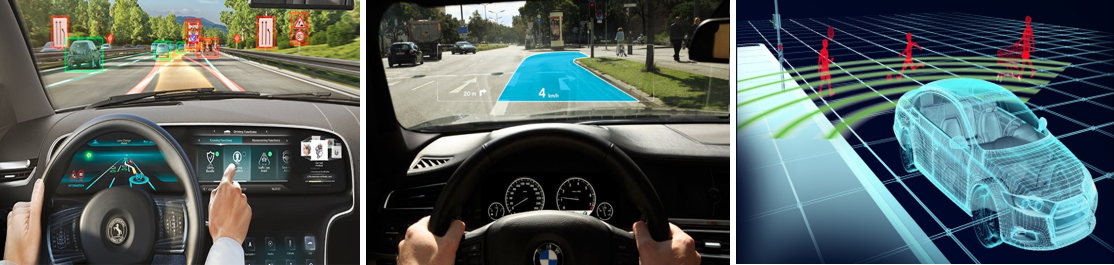
\includegraphics[scale=0.5]{sp.png}
        \caption{Systèmes d'assistance intelligents des voitures}
        \label{fig:systeme intelligents}
\end{figure}
  
\subsection{Véhicules autonomes}

La reconnaissance des panneaux fait partie des fonctions des véhicules autonomes, capable de rouler sans l'intervention d'un conducteur(Figure-\ref{fig:vehicule autonomes}).\\

\begin{figure}[h]
        \centering
        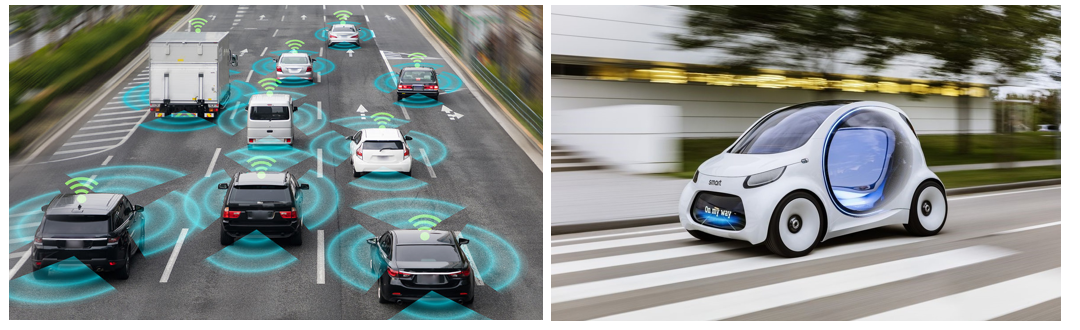
\includegraphics[scale=0.5]{images/tt.png}
        \caption{Véhicules autonomes}
        \label{fig:vehicule autonomes}
\end{figure}
       
\section{Processus de reconnaissance}

Avant de faire la reconnaissance, une étape de détection est d'abord nécessaire (Figure-\ref{fig:processus de}) \cite{10}, ou l’image est pré-traitée, améliorée et segmentée en fonction des propriétés du signe telles que sa couleur ou sa forme. La sortie est une image segmentée contenant des régions potentielles qui pourraient être reconnues comme des panneaux de signalisation possibles.\\

Après cela, vient l’étape de reconnaissance ou chacun des candidats est testé par rapport à un ensemble de fonctionnalités (un modèle) pour décider s’il s’agit ou non d'un panneaux de signalisation, puis selon ces caractéristiques, nous les classons dans différents catégories ou des classes  ou il serait facile de décider de la signification du signe considéré \cite{10}.\\
 
  \begin{figure}[h!]
        \centering
        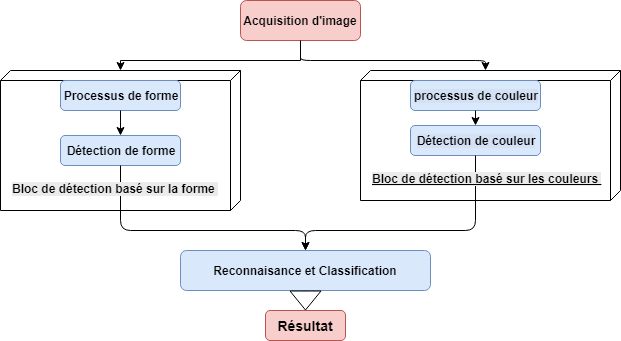
\includegraphics[width=12cm,height=7cm]{yy.png}
        \caption{Processus de détection et de reconnaissance automatique}
        \label{fig:processus de}
\end{figure}
\newpage
Pour mieux expliquer le processus visé par notre travail, la Figure- \ref{fig:schma} présente un schéma typique d’un système de reconnaissance de panneaux routiers. La détection recherche dans les images fournies par une caméra les zones où se trouvent potentiellement des panneaux  (à l’aide d’informations de couleurs, de formes, etc.). Ensuite,un algorithme de reconnaissance permet d’éliminer les régions inutiles et de garder l'information essentielle.\\
\begin{figure}[h]
        \centering
        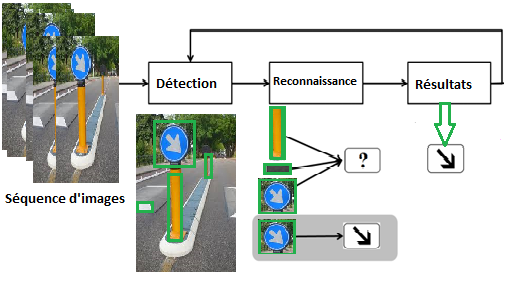
\includegraphics[width=12cm,height=7cm]{images/proces.png}
        \caption{Schéma typique d’un système de reconnaissance}
        \label{fig:schma}
        \end{figure}
\newpage     
\section{Difficultés potentielles  }
Compte tenu de la complexité de l’environnement routier et des scènes qui l'entourent, les panneaux routiers peuvent se trouver dans différentes situations (les exemples de Figure \ref{fig:problemes}), et par conséquent, la détection et la reconnaissance de ces signes peut être entravée par les difficultés suivantes \cite{10} :
\begin{enumerate}
  \item Conditions d’éclairage, qui sont variables et non contrôlables (Figure \ref{fig:problemes} (a),(c));
  \item Présence d'obstacles (Figure \ref{fig:problemes} (d),(e)) ;
  \item L'état physique d'un signe change en fonction de son âge, des accidents, etc (Figure \ref{fig:problemes} (f)) ;
  \item Vu qu’il existent beaucoup de degrés de liberté, la taille de l'objet dépend de la distance à la caméra. l'échelle pour chaque axe est différente (par exemple quand l'axe optique de la caméra n'est pas perpendiculaire au signe), ce qui entraîne une modification de l'aspect de la caméra (Figure \ref{fig:problemes} (g)).
  
 \subsection{Système d'acquisition}
La fonction fondamentale du système d’acquisition est de capturer l'image ou la vidéo afin qu'elle puisse être traitée ultérieurement. La position et la résolution des caméras acquérant les images de signes sont la principale préoccupation. Si les caméras sont placées trop loin (Figure \ref{fig:problemes} (b),(e)), l'image capturée sera floue et si la caméra est placée trop près de la plaque, l'image résultante sera de très grande taille. Par conséquent, la distance entre la caméra et la plaque détermine la qualité de l'image.
 \end{enumerate}
 
 \begin{figure}[h]
        \centering
        \begin{subfigure}
            \centering
            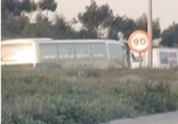
\includegraphics[width=4.2cm,height=4cm]{images/a.png} 
            \caption{(a)}
        \end{subfigure}
        \begin{subfigure}
            \centering
            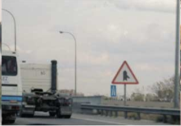
\includegraphics[width=4.2cm,height=4cm]{images/b.png} 
            \caption{(b)}
        \end{subfigure}
        \begin{subfigure}
            \centering
            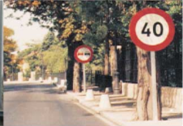
\includegraphics[width=4.2cm,height=4cm]{images/c3.png} 
            \caption{(c)}
        \end{subfigure}
        \begin{subfigure}
            \centering
            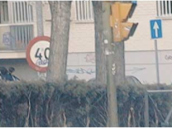
\includegraphics[width=4.2cm,height=4cm]{images/d.png} 
           \caption{(d)}
        \end{subfigure}
        \begin{subfigure}
            \centering
            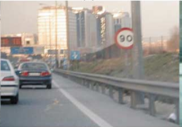
\includegraphics[width=4.2cm,height=4cm]{images/e.png} 
            \caption{(e)}
        \end{subfigure}
        \begin{subfigure}
            \centering
            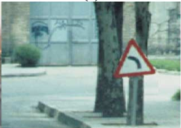
\includegraphics[width=4.2cm,height=4cm]{images/f.png} 
            \caption{(f)}
        \end{subfigure}
        \begin{subfigure}
            \centering
            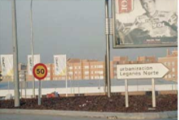
\includegraphics[width=4.2cm,height=4cm]{images/g.png}
            \caption{(g)}
        \end{subfigure}
        \caption{Problèmes rencontrés lors de la  détection et la reconnaissance }
        \label{fig:problemes}
\end{figure}
  \newpage
\section{Conclusion}
Dans ce chapitre, nous avons vu quelques notions fondamentales concernant les classes de panneaux de signalisation routière, les problèmes de normalisation malgré la conventions de Vienne et leurs différents domaines d’application pour montrer l’impact de ce travail et son importance sur la route. Nous avons aussi exposé quelques difficultés qui entravent la détection et la reconnaissance de panneaux de signalisation routière.
%%% Local Variables: 
%%% mode: latex
%%% TeX-master: "../phdthesis"
%%% End: 
